\documentclass[main.tex]{subfiles}

\begin{document}

\chapter{Preassembly}\label{chapter:preassembly}

% Assembly are based on :
% - reads, reads contains error, this error isn't rept
% - overlaps
Assembly tools are based on reads. If your reads are bad, your assembly will be bad. To continue on the analogy given in the introduction, you probably cannot reconstruct a book if crazy monks gave to you only fragments with half of the letters being erroneous. Correction of reads, with a mix of sequencing technologies (or with a single technology), can help you to get better reads. But actually, correction tools have an important cost in term of computation time and memory usage. Moreover it's hard to differentiate natural mutations (e.g. real SNPs) to sequencing errors, and sometimes interesting mutations are consider as errors and are corrected (thus removed).

With long-reads, reads contain many errors. These errors are not quite uniformly distributed along the read \cite{blog_post_error_repartition}. This makes it more difficult to search overlaps between reads. Current techniques attempt to optimize results on real data \cite{ovl_bench}.
Actually, a key observation is that within the overlaps found by state-of-the-art tools, not all of them are useful to downstream analysis. For example \miniasm keeps only end-to-end overlaps, and \canu keeps only the two longest end-to-end overlaps for each read (see \ref{chapter:sota} for more details).

Our paper "\yacrd and \fpa: upstream tools for long-read genome assembly" presents two tools, \yacrd (for Yet Another Chimeric Read Detector), and \fpa (for Filter Pairwise Alignment). \yacrd focuses on the detection and elimination of very poor quality regions. \fpa focuses on filtering 'useless' overlaps.

Having better-quality reads and no unnecessary overlaps can help quickly produce high-quality assemblies. But if overlapping tools miss an important overlap, assembly can be fragmented.
In \cite{ovl_bench}, \citeauthor{ovl_bench} compare the state of the art of overlappers on simulated datasets and on real datasets. A drop in the accuracy and recall of these algorithms can be observed between real and simulated data \ref{preassembly:tab:ovl_result}.

\begin{table}[ht]
    \centering
    \begin{tabular}{l|rr|rr}
                & \multicolumn{2}{c}{Pacbio}                & \multicolumn{2}{c}{Nanopore}              \\ 
                & Simulated           & Real                & Simulated         & Real                  \\ \hline
    Sensibility & 88.9$^m$ - 92.4$^d$ & 59.6$^m$ - 83.8$^d$ & 90.4$^g$ - 95.2$^b$ & 88.9$^b$ - 92.9$^d$ \\
    Precision   & 81.9$^b$ - 96.5$^g$ & 79.8$^h$ - 96.5$^b$ & 75.1$^b$ - 99$^m$   & 73$^b$ - 95.4$^m$   \\
    \end{tabular}
    \caption{\textsuperscript{m}\toolsname{Minimap}, \textsuperscript{d}\toolsname{Daligner}, \textsuperscript{g}\toolsname{GraphMap}, \textsuperscript{b}\toolsname{BLASR}, \textsuperscript{h}\mhap}
    \label{preassembly:tab:ovl_result}
\end{table}

In the blog post "State-of-the-art long reads overlappers comparison" \footnote{\url{https://blog.pierre.marijon.fr/long-reads-overlapper-compare/}} we take  the same data as \cite{ovl_bench} but we didn't care if the overlappers found 'right' or 'wrong' overlaps. Instead we search if they found the same overlaps. There were differences large enough to justify the idea of creating an overlap 'reconciliation' step. A prototype was created by a master student. 
This blog post was present as poster during JOBIM (Journée Ouverte de Bioinformatique \& Mathematique) 2018.

In this chapter we present first \yacrd and \fpa, in the form of a publication that has been sent to a journal. And finally, we mention our work on overlappers consensus.

\subfile{paper/yacrd_fpa.tex}
%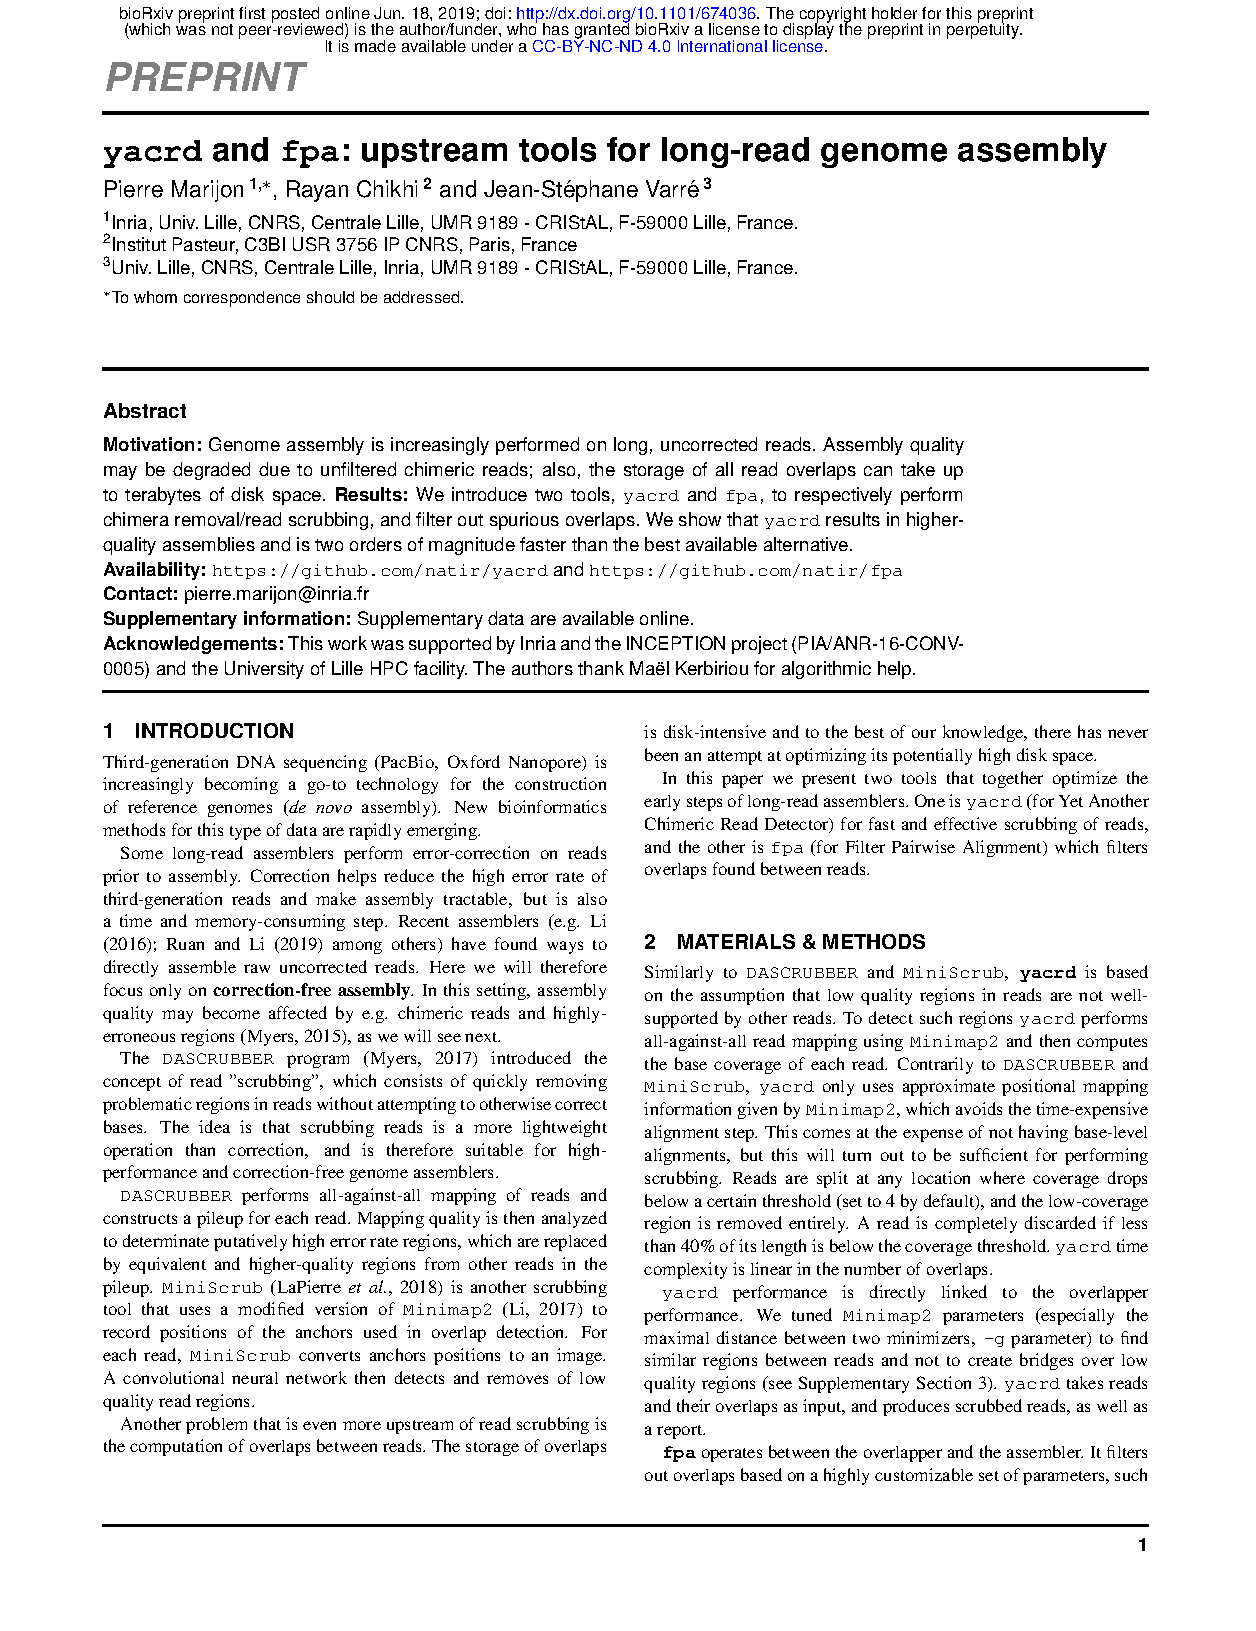
\includepdf[pages=-]{paper/yacrd_fpa.pdf}


\section{Overlapping consensus}\label{section:preassembly:ovl_consensus}

This work begin as an extension of a \citeauthor{bench_ovl} publications \cite{bench_ovl}. Author creaete a benchmark of overlapping tools, they compare \mhap, \minimap, \toolsname{Blasr}\cite{blasr}, \toolsname{Daligner}\cite{daligner} and \toolsname{Graphmap}\cite{graphmap}. This tools was compare on computation time memory usage, sensibility and precision on simulated and real dataset.

An interesting result was a lost of precision and recall between synthetic and real dataset until 25 \% of sensibility for \toolsname{Blasr} on pacbio data. This tools miss some overlap but they miss same overlap ? To answer to this question we write a blog post with some set analysis.

\subfile{paper/blog_post.tex}

\section{Conclusion}

\yacrd and \fpa have an important impact on assembly of \miniasm and \wtdbg. They were well received by the community\yacrd and \fpa was actually used, in some tools and pipeline.

For my blog post on overlapping tools comparaison, this preliminary work was continued within the context of a PFE (\textit{Projet de Fin d'Étude} End of Study Projects) with Yann Grabe who created a tool that will build a consensus of several overlap files. For the moment this tool is only a prototype and would still require a lot of work before it can be finalized. Moreover, the interest of a it tools in the context of assembly seems to be reduced indeed more and more assembly tools mix the overlap research and graph construction part. We can see this evolution in the next chapter of this document where we describe some long read assembly pipeline.


\onlyinsubfile{
\bibliographystyle{plainnat}
\bibliography{main}
\addcontentsline{toc}{chapter}{Bibliography}
}

\end{document}